% BANZA Whitepaper v1.0 — PT edition. Generated from content/pt.json (single source).
\PassOptionsToPackage{table}{xcolor}

%% 2-column papers and preprints
\documentclass[journal abbreviation, manuscript]{copernicus}
\PassOptionsToPackage{portuguese}{babel}
%\documentclass{copernicus}
\usepackage{textcomp}
\usepackage{listings}
\usepackage{savesym}
\usepackage{amsmath}
\savesymbol{unit}
\usepackage{float}
\usepackage{multicol}
\usepackage{siunitx}
\usepackage{todonotes}
\newcounter{todocounter}
\newcommand{\todonum}[2][]{\stepcounter{todocounter}\todo[#1]{\thetodocounter: #2}}
\usepackage{cancel}
% (integration) [table]{xcolor} is passed via \PassOptionsToPackage before the class — see line 1
\usepackage{colortbl}        % for coloring cells, rows, columns
\usepackage{booktabs}        % for nicer horizontal lines (\toprule, etc.)
%\title{BANZA: Protocolo Aberto de Interoperabilidade Financeira}
%\author{Fidel R. Monteiro \and Jesus R. Monteiro}
%\date{1 de agosto de 2026}
%\usepackage[portuguese]{babel}
\renewcommand{\abstractname}{Resumo}
\newcommand{\blfootnote}[1]{%
  \begingroup
  \renewcommand{\thefootnote}{}%
  \footnotetext{#1}%
  \addtocounter{footnote}{-1}%
  \endgroup
}
\makeatletter
\def\@@and{e}
\makeatother
%\emergencystretch=2em


\begin{document}
\selectlanguage{portuguese}
% (integration) ini-based babel locales (XeTeX/tectonic) lack these captions; restore the approved ones:
\renewcommand{\abstractname}{Resumo}
\renewcommand{\refname}{Referências}
\renewcommand{\figurename}{Figura}
\renewcommand{\tablename}{Tabela}
\title{BANZA: Protocolo Aberto de Interoperabilidade Financeira}

\Author[1][contact@banza.network]{Fidel}{R.~Monteiro}
\Author[1]{Jesus}{R.~Monteiro}

\affil[1]{%
 BANZAMI -- Tecnologia e Serviços, Lda., Luanda, Angola%
\protect\newline
Website oficial: \url{https://banza.network}%
}



\runningtitle{BANZA: Protocolo Aberto de Interoperabilidade Financeira}
\runningauthor{Monteiro and Monteiro}
\received{}
\pubdiscuss{} %% only important for two-stage journals
\revised{}
\accepted{}
\published{10-08-2026}

%% These dates will be inserted by Copernicus Publications during the typesetting process.

\firstpage{1}

\maketitle
\nolinenumbers

\begin{abstract}
Operadores financeiros independentes interoperam através de integrações bilaterais e de infraestruturas partilhadas, mas as especificações, os testes e os resultados nem sempre são públicos, dificultando a reprodução da validação técnica. Este artigo apresenta o BANZA, um protocolo aberto de interoperabilidade financeira baseado em regras públicas e versionadas, validação determinística e evidência verificável. O modelo avalia implementações segundo versões e perfis públicos, separa protocolo, certificação e esquemas operacionais e liga cada resultado às entradas que o produziram através de artefactos canónicos, resumos criptográficos, códigos de motivo e recibos. Desta forma, a conformidade técnica pode ser inspeccionada, reproduzida e verificada por terceiros. O protocolo e a implementação de referência permanecem em pré-produção; por isso, desempenho, escalabilidade, adopção e comportamento em ambientes operacionais reais ainda não foram demonstrados experimentalmente.
\end{abstract}

\begingroup
\renewcommand{\thefootnote}{\fnsymbol{footnote}}
\footnotetext[1]{%
\textit{A edição em língua portuguesa constitui a versão canónica do Whitepaper do BANZA. A edição em língua inglesa é uma tradução oficial. Em caso de divergência não intencional, prevalece a edição canónica em português.}%
}
\endgroup



\section{Introdução}\label{sec:introduction}

Os operadores financeiros raramente funcionam de forma isolada. Para trocar valor ou mensagens, as respectivas implementações precisam de acordar formatos, mecanismos de identidade, chaves, semântica de erros e procedimentos de teste. Em integrações bilaterais, estes elementos são definidos entre cada par de operadores; quando especificações, testes e resultados permanecem privados, o trabalho pode ser repetido e a validação técnica torna-se difícil de reproduzir por terceiros.

Seja \(n\) o número de operadores. As Equações \eqref{eq:bilateral} e \eqref{eq:common} representam, respectivamente, uma malha de integrações bilaterais e a adopção de um protocolo comum.

\begin{align}
R_{\text{bilateral}}(n) &= \frac{n(n-1)}{2} \tag{1a}\label{eq:bilateral} \\
I_{\text{comum}}(n) &= n \tag{1b}\label{eq:common}
\end{align}

A Equação \eqref{eq:bilateral} conta as relações técnicas entre pares de operadores, enquanto a Equação \eqref{eq:common} conta as implementações necessárias quando cada operador adopta o protocolo comum. Assim, a entrada de um novo operador pode exigir até \(n\) novas integrações bilaterais, mas apenas uma nova implementação do protocolo. A Figura \ref{fig:bilateral} ilustra os dois regimes.

\begin{figure}[H]
  \centering
  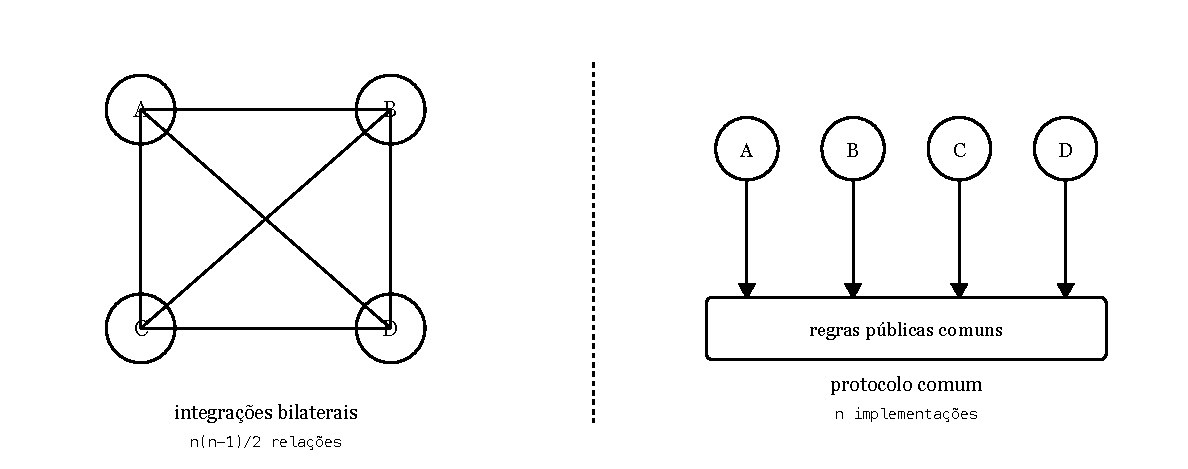
\includegraphics[
    width=1\linewidth,
    trim={0cm 0.3cm 0cm 1cm},
    clip
  ]{figures/fig1-bilateral-vs-protocol.pt.pdf}
  \caption{Comparação entre uma malha bilateral completa, com \(n(n-1)/2\) relações técnicas, e um protocolo comum, com \(n\) implementações, uma por operador.}
  \label{fig:bilateral}
\end{figure}

A interoperabilidade também pode ser assegurada por infraestruturas partilhadas e centralizadas. Estes modelos permitem a operação entre participantes, mas as suas especificações, testes e resultados nem sempre estão disponíveis de forma que permita uma reprodução independente. O BANZA não procura substituir essa interoperabilidade operacional: acrescenta uma camada aberta de especificações, perfis e contratos públicos e versionados, conformidade determinística e evidência verificável e reproduzível.

Normas como a ISO 20022 [1], a ISO 8583 [2], as especificações EMV para pagamentos por QR [3] e a ISO/IEC 9646 [4] tratam de componentes relevantes de mensagens, pagamentos e testes de conformidade. O BANZA complementa estes trabalhos ao definir um protocolo aberto no qual cada implementação publica artefactos na sua origem canónica, é avaliada segundo uma versão e um perfil públicos e produz resultados ligados às entradas observadas. A avaliação incide sobre implementações, e não sobre entidades, mantendo separados o protocolo, a certificação e os esquemas operacionais.

Este documento é fundacional e não normativo. \S\ref{sec:model} e \S\ref{sec:architecture} apresentam o modelo e a arquitectura do BANZA; \S\ref{sec:profiles}, os perfis de conformidade; \S\ref{sec:discovery}, os mecanismos de descoberta, identidade e confiança; e \S\ref{sec:validation} e \S\ref{sec:evidence}, a validação e a evidência. A segurança e a governação são tratadas em \S\ref{sec:security} e \S\ref{sec:governance}; as limitações e o estado actual, em \S\ref{sec:limitations} e \S\ref{sec:state}; e \S\ref{sec:conclusion} apresenta as conclusões.


\section{Modelo}\label{sec:model}

O BANZA distingue um operador de uma implementação. Um operador é a entidade organizacional responsável; uma implementação é o sistema técnico avaliado, e um mesmo operador pode publicar várias implementações --- de demonstração, de teste, de pré-produção ou de produção. Qualquer resultado de validação ou certificação aplica-se sempre a uma implementação, versão do protocolo, perfil, ambiente, âmbito, conjunto de evidências e período de validade determinados, e nunca a uma entidade em abstracto. Cada implementação tem um identificador estável, e o conjunto exacto de artefactos avaliados --- a versão construída --- é fixado por um resumo criptográfico de conteúdo. Uma versão construída diferente constitui um sujeito de avaliação distinto, ainda que pertença à mesma implementação, e exige a sua própria avaliação.

Modelamos uma implementação como um tuplo de seis elementos. Na Equação \eqref{eq:tuple}, \(o\) identifica o operador, \(i\) a implementação, \(v\) a versão do protocolo, \(p\) o perfil de conformidade, \(e\) o ambiente e \(u\) a origem canónica.

\begin{equation}
\mathcal{I} = (o,\, i,\, v,\, p,\, e,\, u)
\tag{2}\label{eq:tuple}
\end{equation}

Os artefactos observados na origem num dado instante \(t\) formam um conjunto. A Equação \eqref{eq:artifacts} representa esse conjunto, em que \(n\) corresponde ao número de artefactos.

\begin{equation}
A_t(\mathcal{I}) = \{\, a_1,\, a_2,\, \dots,\, a_n \,\}
\tag{3}\label{eq:artifacts}
\end{equation}

A validação toma esses artefactos e a especificação aplicável \(S\) para a versão \(v\) e o perfil \(p\). A Equação \eqref{eq:validation} descreve este processo. A avaliação é executada pela versão do motor \(m\) e produz o resultado \(R\), a evidência \(E\) e os recibos \(P\). Neste modelo, \(R\) compreende o veredicto e o código de motivo que o fundamenta.

O âmbito é, por isso, explícito e não implícito: um resultado declara o perfil face ao qual foi avaliado, a versão do protocolo considerada, o ambiente da execução e a evidência consumida. É válido apenas para essa combinação e nunca generaliza silenciosamente do artefacto avaliado para a entidade que o publicou. A reprodutibilidade é uma propriedade de primeira classe: dadas entradas canónicas equivalentes, a mesma especificação, o mesmo perfil e a mesma versão do motor, execuções independentes produzem veredictos e códigos de motivo semanticamente equivalentes [8]. Os metadados não determinísticos, como as marcas temporais de execução, são excluídos desta equivalência.

\begin{equation}
V_m\!\left(A_t(\mathcal{I}),\, S_{v,p}\right) \rightarrow (R,\, E,\, P)
\tag{4}\label{eq:validation}
\end{equation}

\begin{figure}[H]
  \centering
  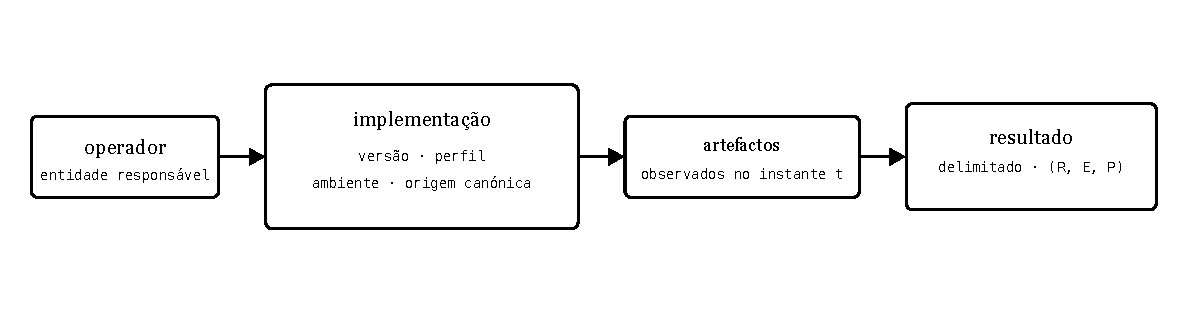
\includegraphics[width=1\linewidth, trim={0.cm 1.5cm 0.cm 1.2cm}]{figures/fig2-model.pt.pdf}
  \caption{Um operador publica uma implementação com uma versão, um perfil, um ambiente e uma origem canónica; os artefactos observados nessa origem são avaliados e produzem um resultado válido apenas para essa combinação.}\label{fig:model}
\end{figure}

Os resumos criptográficos de conteúdo, calculados com SHA-256 [5], permitem identificar e comparar exactamente as entradas observadas. Em conjunto com a disponibilidade dessas entradas, transformam «foi validado» em «qualquer pessoa pode revalidá-lo». A Figura \ref{fig:model} relaciona o operador, a implementação e os seus atributos com os artefactos observados e o resultado delimitado.


\section{Arquitectura}\label{sec:architecture}

O BANZA organiza-se em três camadas institucionais, separadas por responsabilidade, infraestrutura e chaves. A Camada 1 corresponde ao protocolo aberto e reúne as regras, contratos e mecanismos comuns de descoberta, identidade, confiança, revogação e federação. A Camada 2 avalia implementações face a perfis e versões públicas através de motores determinísticos em Rust. A Camada 3 compreende esquemas operacionais independentes que podem adoptar o BANZA e permanecem sujeitos ao enquadramento jurídico e regulatório aplicável.

\begin{figure}[H]
  \centering
  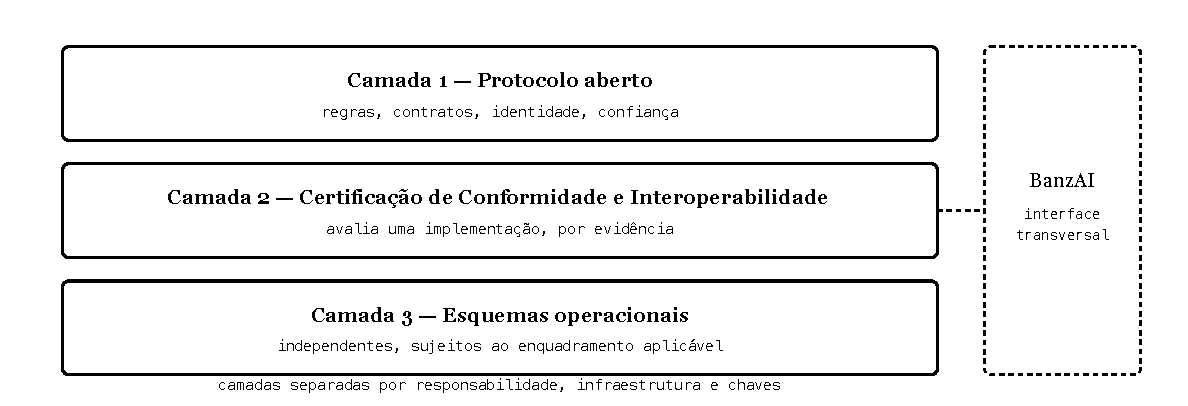
\includegraphics[width=1\linewidth, trim={0cm 0.2cm 0cm 0.5cm}, clip]{figures/fig3-three-layers.pt.pdf}
  \caption{Camada 1, protocolo aberto; Camada 2, certificação por implementação; Camada 3, esquemas operacionais independentes. O BanzAI é uma interface transversal às três, não uma quarta camada nem uma autoridade.}
  \label{fig:layers}
\end{figure}

A separação das camadas preserva a neutralidade do protocolo: todas as implementações são avaliadas segundo os mesmos perfis, motores e modelo de evidência. Certificação técnica, admissão num esquema e autorização regulatória são determinações independentes. O BanzAI funciona como interface humana para consulta e explicação dos resultados, sem participar na decisão; os consumidores automáticos acedem directamente às interfaces públicas. A Figura \ref{fig:layers} resume esta arquitectura. Os perfis L0--L4, apresentados em \S\ref{sec:profiles}, são distintos das três camadas.

\section{Perfis}\label{sec:profiles}

O BANZA define cinco níveis cumulativos de conformidade, de L0 a L4. A adopção técnica passa pela escolha de um perfil, pela publicação dos artefactos na origem canónica e pela execução da jornada de validação. Um resultado positivo num nível constitui evidência técnica de interoperabilidade, não uma certificação, autorização ou aprovação.

O nível L0 --- Protocol Sandbox --- valida a configuração segura do protocolo em ambiente de testes, com manifesto válido e representação monetária correcta. O L1 --- Core Payment Capability --- acrescenta capacidades essenciais de pagamento e rastreabilidade. O L2 --- Payment Initiation Capability --- acrescenta iniciação de pagamentos por pedido ou por código QR dinâmico. O L3 --- Inter-Operator Interoperability --- acrescenta interoperabilidade entre operadores, incluindo liquidação e reconciliação, constitui o limiar de elegibilidade para federação e exige evidência multi-operador. O L4 --- External Interoperability --- acrescenta integração com redes externas; é definido por perfil e exige evidência específica dessa integração.

Os níveis L0 a L2 podem ser aferidos num único operador, enquanto L3 e L4 exigem, respectivamente, evidência de federação e de integração externa. Um perfil de certificação é distinto destes níveis: fixa um nível de conformidade e o conjunto de capacidades, esquemas, contratos e pontos de acesso exigidos. A Figura \ref{fig:profiles} resume a progressão cumulativa e o que cada nível acrescenta.

\begin{figure}[H]
  \centering
  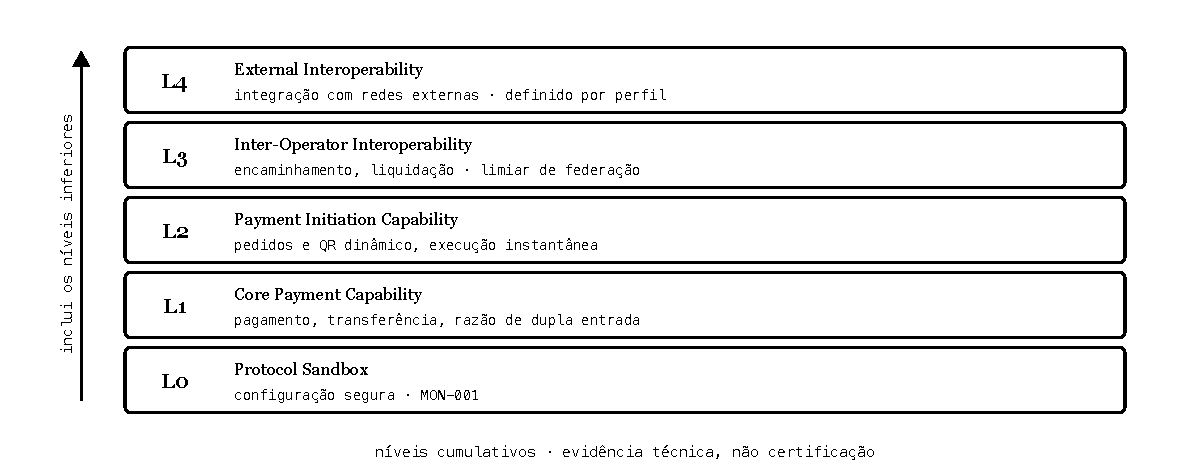
\includegraphics[width=1\linewidth,trim={0cm 0.2cm 0cm 0.5cm},clip]{figures/fig4-profiles.pt.pdf}
  \caption{Cada nível inclui todos os inferiores e acrescenta capacidades; L3 é o limiar de elegibilidade para a federação e L4 é definido por perfil, com evidência de integração externa.}\label{fig:profiles}
\end{figure}


\section{Descoberta}\label{sec:discovery}

Cada implementação publica os seus artefactos numa origem canónica controlada pelo operador [7]. A descoberta começa num caminho fixo sob essa origem e devolve um Manifesto com a identificação da implementação, os pontos de acesso, a versão do protocolo, o perfil declarado, os metadados assinados e as chaves públicas. O Registo Técnico associa o operador, a implementação e a origem canónica, e todos os pontos de acesso anunciados devem pertencer a essa origem.


\begin{figure}[H]
  \centering
  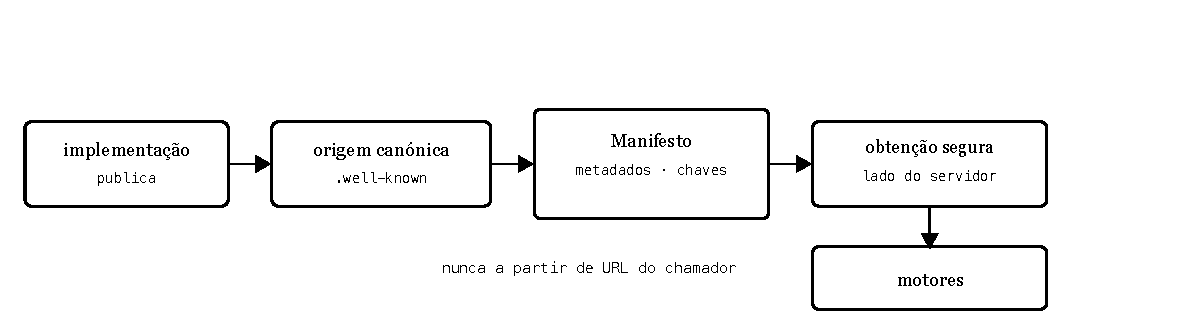
\includegraphics[width=1\linewidth,trim={0cm 0.3cm 0cm 1.7cm},clip]{figures/fig5-discovery.pt.pdf}
  \caption{Uma implementação publica artefactos assinados na origem canónica que o operador controla; um módulo de obtenção segura, do lado do servidor, obtém o Manifesto e as chaves e entrega-os aos motores, nunca a partir de uma URL fornecida pelo chamador.}\label{fig:discovery}
\end{figure}

A identidade e a integridade assentam em chaves publicadas e metadados assinados. Uma raiz de confiança, mantida fora de linha, assina o Manifesto de Chaves com Ed25519 [6]; essa assinatura é a base para confiar nas chaves emissoras. As chaves são separadas por domínio, e a revogação permite detectar material revogado, substituído ou expirado.

Os motores obtêm os artefactos do lado do servidor através de um módulo de obtenção segura, que resolve o alvo a partir do registo e nunca segue uma URL fornecida pelo chamador. A Figura \ref{fig:discovery} resume este percurso.


\section{Validação}\label{sec:validation}

A validação segue uma jornada fixa de oito passos técnicos e um passo final de agregação. Cada passo é executado por motores determinísticos em Rust e recebe um de quatro estados: verificado, pendente, falhado ou bloqueado. A avaliação adopta fecho por omissão: evidência ausente, expirada ou inconsistente nunca produz aprovação. A prontidão para certificação só é atingida quando todos os passos técnicos estão verificados, mas não constitui, por si só, uma certificação.

A decisão permanece separada da explicação. Os motores determinísticos produzem os resultados, enquanto o BanzAI apenas os apresenta e explica, sem os alterar ou decidir. A certificação técnica é um processo distinto, que associa formalmente uma implementação a um perfil público versionado. A Figura \ref{fig:journey} resume a jornada, os estados e separação.

\begin{figure}[H]
  \centering
  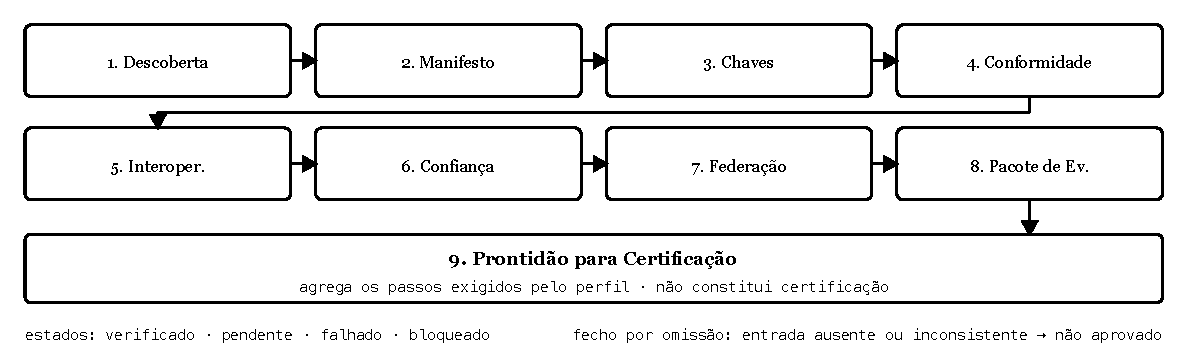
\includegraphics[width=1\linewidth,trim={0cm 0.5cm 0cm 0.5cm},clip]{figures/fig6-journey.pt.pdf}
  \caption{Oito passos técnicos e um passo de agregação; cada passo recebe um estado com códigos de motivo e falha por omissão; a prontidão para certificação só é atingida quando todos os passos técnicos estão verificados e nunca devolve um veredicto de certificação.}
  \label{fig:journey}
\end{figure}

A Figura \ref{fig:example} mostra um exemplo entre dois operadores: B publica os seus artefactos, A inicia a avaliação e os motores produzem resultados, recibos e evidência verificável. O BANZA fornece a base técnica da decisão, mas cabe ao Operador A decidir, segundo a sua própria política, se o resultado satisfaz as suas necessidades.

\begin{figure}[H]
  \centering
  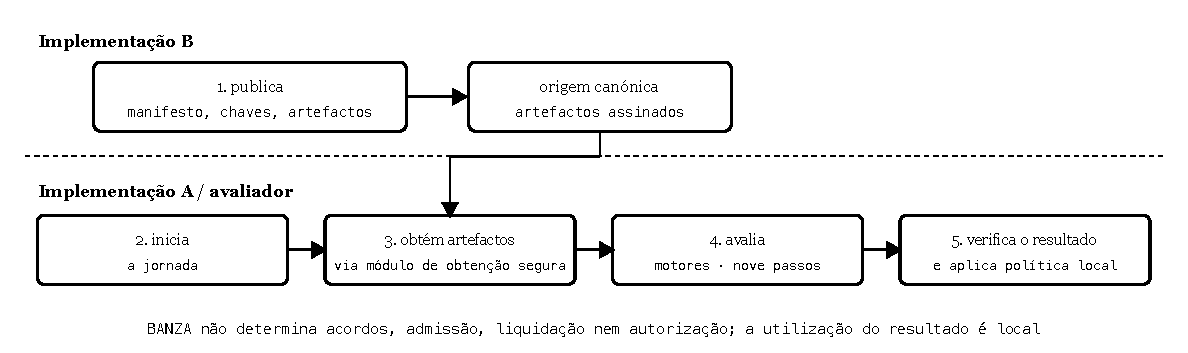
\includegraphics[width=1\linewidth,trim={0cm 0.5cm 0cm 0.5cm},clip]{figures/fig7-example.pt.pdf}
  \caption{O Operador B publica os artefactos na sua origem canónica; o Operador A, ou um avaliador, inicia a jornada; o módulo seguro obtém os artefactos, os motores validam e produzem resultados, recibos e evidência; o Operador A verifica ou reproduz o resultado e decide, sob a sua própria política.}
  \label{fig:example}
\end{figure}


\section{Evidência}\label{sec:evidence}

Cada validação produz resultados, recibos e evidência verificável. Os recibos registam os passos executados e ligam cada resultado à versão do protocolo, ao perfil, aos artefactos consumidos, aos respectivos resumos criptográficos e aos códigos de motivo, permitindo confirmar ou reproduzir a base técnica da avaliação (Figura \ref{fig:evidence}).

\begin{figure}[H]
  \centering
  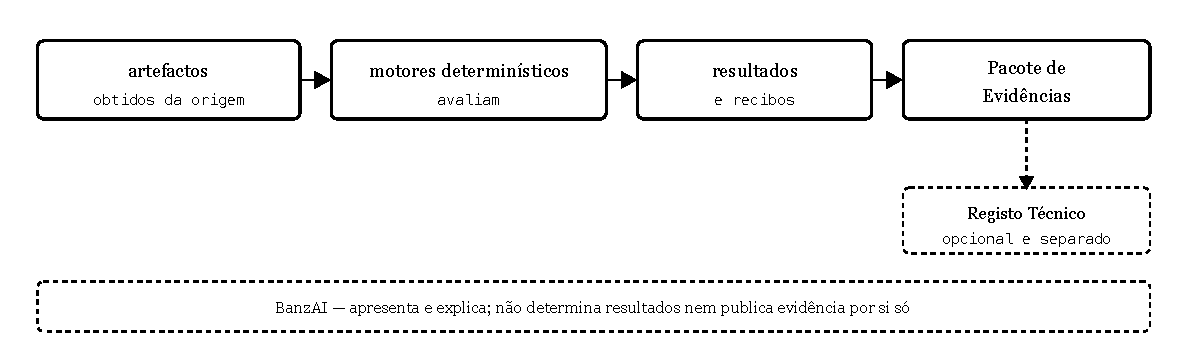
\includegraphics[width=1\linewidth,trim={0cm 0.6cm 0cm 0.9cm},clip]{figures/fig8-evidence.pt.pdf}
  \caption{Os artefactos entram nos motores, que decidem e emitem resultados; os resultados tornam-se recibos e um Pacote de Evidências; a publicação no Registo Técnico é opcional e separada; o BanzAI apenas apresenta e explica.}
  \label{fig:evidence}
\end{figure}

Um recibo representa o estado observado no instante da avaliação; alterações posteriores aos artefactos exigem nova avaliação. O Pacote de Evidências reúne os artefactos e referências que sustentam o resultado, mas não constitui certificação nem concede qualquer estado operacional.

A publicação é separada da avaliação. Os resultados podem ser publicados no Registo Técnico, uma superfície pública de leitura que indexa metadados e evidência verificável. A ausência de uma entrada não constitui proibição, e qualquer terceiro pode reexecutar a avaliação a partir dos artefactos publicados.


\section{Segurança}\label{sec:security}

O modelo de ameaças considera adulteração de artefactos, origens ou chaves inválidas, repetição de desafios, evidência expirada ou incompleta e divergências de versão. Na obtenção remota, inclui ainda SSRF e reassociação de DNS. O BANZA responde com assinaturas, revogação, expiração, desafios de uso único e avaliação com fecho por omissão, na qual entradas ausentes ou inconsistentes não são aprovadas (Figura \ref{fig:security}).

\begin{figure}[H]
  \centering
  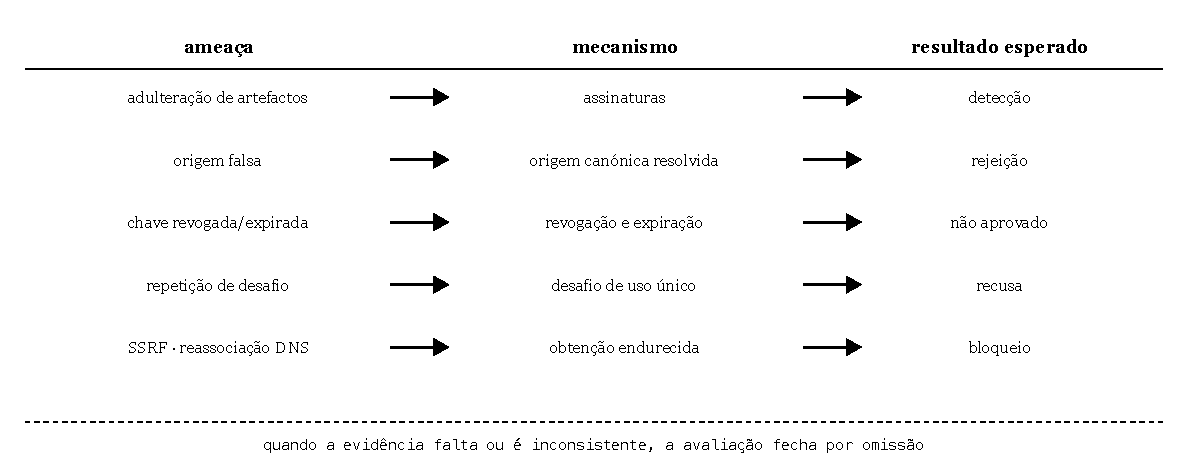
\includegraphics[width=1\linewidth,trim={0cm 0.3cm 0cm 0.3cm},clip]{figures/fig9-security.pt.pdf}
  \caption{Cada ameaça considerada corresponde a um mecanismo de protecção e a um resultado esperado; entradas ausentes ou inconsistentes conduzem à não aprovação, por fecho por omissão.}
  \label{fig:security}
\end{figure}

O módulo de obtenção segura é o único componente que acede aos pontos de acesso do operador. O alvo é sempre resolvido a partir da origem canónica registada, nunca de uma URL fornecida pelo chamador. O módulo aceita apenas HTTPS, bloqueia endereços privados, locais ou de metadados de nuvem, fixa a ligação aos endereços validados e não segue redireccionamentos. Também valida TLS e limita as respostas recebidas.


\section{Governação}\label{sec:governance}

O BANZA evolui através de instrumentos públicos de decisão: os ADR registam decisões adoptadas e os RFC propõem alterações ainda em discussão. O protocolo segue versionamento semântico; alterações compatíveis entram em versões menores ou de correcção, enquanto alterações incompatíveis exigem uma nova versão maior. Cada implementação declara a versão e o perfil que adopta, e um perfil de certificação permanece imutável depois de publicado.

\begin{figure}[H]
  \centering
  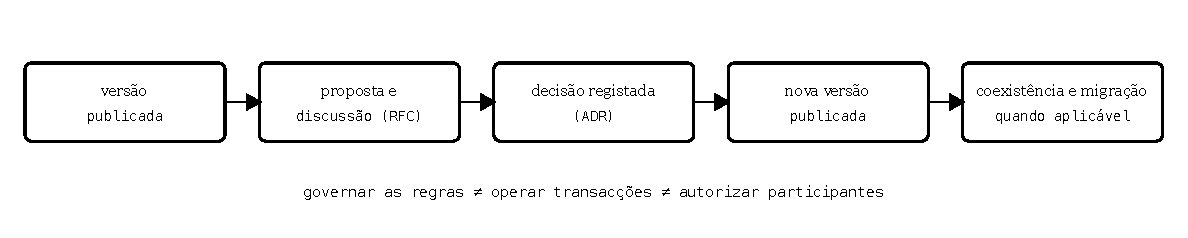
\includegraphics[width=1\linewidth,trim={0cm 0.7cm 0cm 0.2cm},clip]{figures/fig10-governance.pt.pdf}
  \caption{Uma versão actual pode receber alterações aditivas sem ruptura; uma alteração incompatível abre uma versão maior, anunciada como depreciação, com coexistência durante uma janela de transição, migração e, por fim, fim de suporte.}
  \label{fig:governance}
\end{figure}

Alterações incompatíveis são anunciadas antecipadamente e acompanhadas de um caminho de migração, permitindo a coexistência temporária entre versões. A depreciação ocorre de forma explícita e faseada: uma funcionalidade é primeiro marcada como depreciada e só pode ser removida numa versão maior (Figura \ref{fig:governance}). A versão actual do protocolo é a 1.0.

\section{Limitações}\label{sec:limitations}

As garantias do BANZA têm fronteiras claras. Em primeiro lugar, são técnicas e não regulatórias: um resultado positivo demonstra conformidade com um perfil público, mas não implica autorização para operar.

Em segundo lugar, a reprodutibilidade aplica-se apenas aos motores determinísticos sobre as entradas declaradas. Não se estende a propriedades que o protocolo não observa, como os controlos internos de um operador ou o comportamento fora do protocolo. Uma origem ou chave comprometida só pode ser tratada quando existirem sinais observáveis ou uma revogação declarada.

Por fim, a evidência apresentada neste documento é arquitectural. Demonstra o mecanismo numa implementação de referência, mas não mede desempenho, escala ou adopção, que permanecem questões para estudo empírico (Figura \ref{fig:limits}).

\begin{figure}[H]
  \centering
  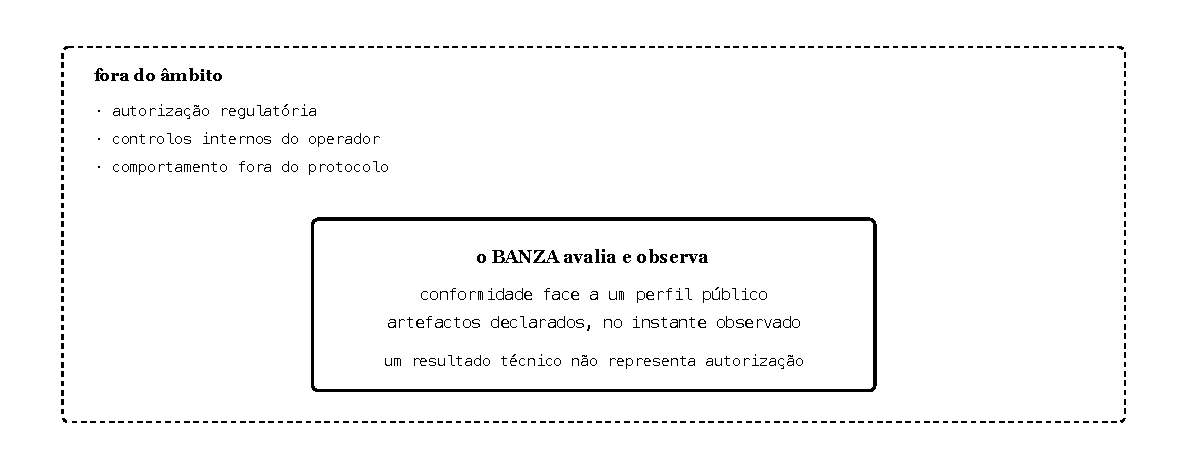
\includegraphics[width=0.9\linewidth, trim={0cm 0.6cm 0cm 0.4cm}, clip]{figures/fig11-limits.pt.pdf}
  \caption{O BANZA avalia a conformidade de uma implementação face a um perfil público e observa os artefactos declarados; permanecem fora do âmbito a autorização regulatória, os controlos internos e o comportamento fora do protocolo, e um resultado técnico não representa nenhum destes.}\label{fig:limits}
\end{figure}


\section{Estado}\label{sec:state}

O BANZA permanece em pré-produção. À data de publicação, o Registo Técnico contém zero operadores de produção e zero certificações técnicas activas; os pagamentos com dinheiro real permanecem desactivados enquanto a camada operacional se encontra em preparação regulatória. Este estado é imposto por um controlo com fecho por omissão em Rust. Não são apresentadas medições de desempenho, e o registo vazio corresponde ao estado actual esperado (Figura \ref{fig:state}).

A implementação de referência, o Operador Zero, funciona num ambiente de testes isolado, em modo de leitura e com moeda de demonstração. Não movimenta fundos reais, permanece não certificada e não destinada à produção, e é avaliada pelos mesmos motores e pela mesma jornada aplicáveis às restantes implementações.

\begin{figure}[H]
  \centering
  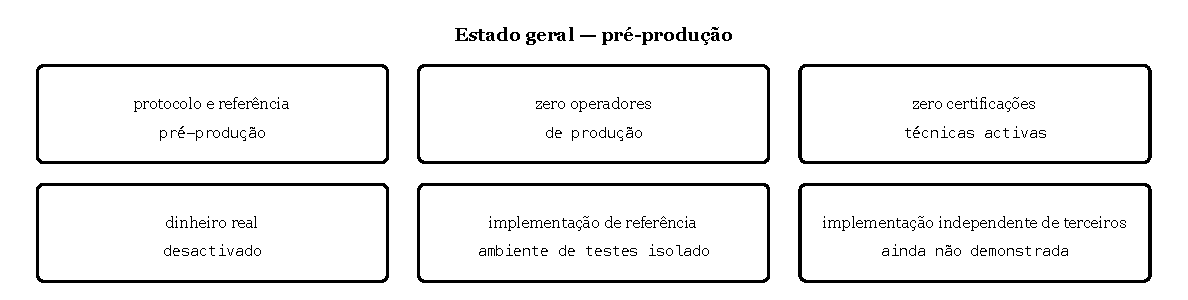
\includegraphics[width=1\linewidth, trim={0cm 0.2cm 0cm 0.4cm}, clip]{figures/fig12-state.pt.pdf}
  \caption{Estado de pré-produção do BANZA: zero operadores de produção, zero certificações técnicas activas, dinheiro real desactivado e uma implementação de referência em ambiente de testes.}
  \label{fig:state}
\end{figure}


\section{Conclusões}\label{sec:conclusion}

Este trabalho apresentou o BANZA como um protocolo aberto de interoperabilidade financeira baseado em regras públicas e versionadas, validação determinística e evidência verificável. O protocolo complementa a interoperabilidade existente com uma base técnica comum que pode ser inspeccionada, reproduzida e verificada por terceiros.

As principais contribuições são:

\begin{itemize}
  \item avaliação de implementações segundo versões e perfis públicos, em vez de entidades em abstracto;

  \item separação entre protocolo, certificação e esquemas operacionais, mantendo distintas a conformidade técnica, a admissão e a autorização regulatória;

  \item validação determinística ligada aos artefactos de entrada através de resumos criptográficos, códigos de motivo, recibos e evidência verificável;

  \item perfis cumulativos de conformidade e uma jornada de validação com estados explícitos e fecho por omissão;

  \item separação entre decisão determinística e explicação assistida pelo BanzAI.
\end{itemize}

As garantias permanecem limitadas ao âmbito técnico observado. A conformidade de uma implementação não constitui autorização para operar, e o actual estado de pré-produção ainda não permite concluir sobre desempenho, escalabilidade ou adopção em ambientes operacionais reais.


O trabalho futuro deverá concentrar-se na medição da reprodutibilidade entre avaliadores independentes e na avaliação do protocolo em cenários multi-operador. Deverá também analisar o desempenho, a escalabilidade, os custos de integração e a evolução dos perfis de conformidade.


Em síntese, o BANZA estabelece uma base aberta e reproduzível para a interoperabilidade financeira, tornando verificáveis as regras, a conformidade e a evidência que sustentam cada implementação. A sua contribuição central é permitir que a interoperabilidade técnica possa ser demonstrada e reproduzida por terceiros.


\begin{thebibliography}{8}
\bibitem{ref1} International Organization for Standardization. ISO 20022 --- Financial services --- Universal financial industry message scheme. ISO. https://www.iso20022.org/
\bibitem{ref2} International Organization for Standardization. ISO 8583:2023 --- Financial-transaction-card-originated messages --- Interchange message specifications. Edition 3. ISO, 2023. https://www.iso.org/standard/79451.html
\bibitem{ref3} EMVCo, LLC. EMV QR Code Specification for Payment Systems (EMV QRCPS): Merchant-Presented Mode, Version 1.1. EMVCo, November 2020. https://www.emvco.com/
\bibitem{ref4} International Organization for Standardization / International Electrotechnical Commission. ISO/IEC 9646-1:1994 --- Information technology --- Open Systems Interconnection --- Conformance testing methodology and framework --- Part 1: General concepts. ISO/IEC, 1994.
\bibitem{ref5} National Institute of Standards and Technology (NIST). Secure Hash Standard (SHS). FIPS PUB 180-4. NIST, August 2015. DOI 10.6028/NIST.FIPS.180-4. https://nvlpubs.nist.gov/nistpubs/fips/nist.fips.180-4.pdf
\bibitem{ref6} S. Josefsson and I. Liusvaara. Edwards-Curve Digital Signature Algorithm (EdDSA). RFC 8032, IRTF, January 2017. DOI 10.17487/RFC8032. https://www.rfc-editor.org/rfc/rfc8032
\bibitem{ref7} M. Nottingham. Well-Known Uniform Resource Identifiers (URIs). RFC 8615, IETF, May 2019. DOI 10.17487/RFC8615. https://www.rfc-editor.org/rfc/rfc8615
\bibitem{ref8} R. Peng. Reproducible Research in Computational Science. Science, 334(6060):1226--1227, 2011. DOI 10.1126/science.1213847. https://doi.org/10.1126/science.1213847
\end{thebibliography}

\end{document}
